\documentclass{article}
\usepackage[tmargin=1in,bmargin=1in,lmargin=1.5in,rmargin=1.5in]{geometry}
\usepackage{amsfonts,amsmath,amssymb,amsthm}
\usepackage{mathrsfs}
\usepackage{ccfonts}
\usepackage{relsize,fancyhdr,parskip}
\usepackage{graphicx}

\usepackage{tikz}
\usetikzlibrary{shapes, shapes.geometric,
  shapes.symbols, shapes.arrows, shapes.multipart, shapes.callouts,
  shapes.misc,decorations.markings,decorations.shapes}

\pagestyle{fancy}
\lhead{Ben Carriel}
\chead{Math 6510 Problem Set 4}
\rhead{\today}

\headheight 13.0pt
\parskip 7.2pt
\parindent 8pt

\newcommand{\tab}{\hspace*{2em}}
\newcommand{\tand}{\tab\text{and}\tab}

\DeclareMathOperator{\N}{\mathbb{N}}
\DeclareMathOperator{\Z}{\mathbb{Z}}
\DeclareMathOperator{\Q}{\mathbb{Q}}
\DeclareMathOperator{\R}{\mathbb{R}}
\DeclareMathOperator{\C}{\mathbb{C}}
\DeclareMathOperator{\D}{\mathbb{D}}
\DeclareMathOperator{\T}{\mathbb{T}}
\DeclareMathOperator{\capchi}{\raisebox{2pt}{$\mathlarger{\mathlarger{\chi}}$}}

%\DeclareMathOperator{\divides}{\mathrel{|}}
\DeclareMathOperator{\suchthat}{\mathrel{:}}

\DeclareMathOperator{\lra}{\longrightarrow}
\DeclareMathOperator{\into}{\hookrightarrow}
\DeclareMathOperator{\onto}{\twoheadrightarrow}
\DeclareMathOperator{\bijection}{\leftrightarrow}
\DeclareMathOperator{\lap}{\bigtriangleup}

\newcommand{\problem}[1]{\noindent{\textbf{Problem #1}}\\}
\newcommand{\problempart}[1]{\noindent{\textbf{(#1)}}}
\newcommand{\exercise}[1]{\noindent{\textbf{Exercise #1:}}}

\newcommand{\der}[2]{\frac{\partial #1}{\partial #2}}
\newcommand{\norm}[1]{\|#1\|}
\newcommand{\diam}[1]{\text{diam}(#1)}
\newcommand{\seq}[2]{\{#1_{#2}\}_{#2 = 1}^\infty}

\newcommand{\conj}[1]{\overline{#1}}
\newcommand{\cis}[1]{\operatorname{cis}#1}
\newcommand{\res}{\operatorname{res}}

\newcommand{\real}{\mathrel{\text{Re}}}
\newcommand{\imag}{\mathrel{\text{Im}}}
\newtheorem*{thm}{\\ Theorem}
\newtheorem*{lem}{\\ Lemma}
\newtheorem*{claim}{\\ Claim}
\newtheorem*{defn}{\\ Definition}
\newtheorem*{prop}{\\ Proposition}

\begin{document}
\exercise{1.3.12} (Drawing attached: Looks like 8 $S^1$'s wedged
together in a loop)

Let $N \leq \pi_1(S^1 \vee S^1)$ be the smallest normal subgroup
generated by $a^2,b^2,(ab)^4$. If we consider the action of $N$ on the
universal cover of $S^1 \vee S^1$, we will identify the orbits of each
of the actions of each of these three generators. I constructed this
Cayley graph iteratively via the following process:
\begin{enumerate}
\item Start at $e$ and add a vertex for each of $a,b$. Add the edges
  $a,b$ to these vertices and then add the reverse edges due to the
  relations $a^2,b^2$ respectively. Proceed to one of the new vertices.
\item Every time we visit a vertex we add new vertices according to
  the action of $a,b$ on the group element corresponding to that
  vertex, subject to the restrictions given by the relations which are
  \begin{enumerate}
  \item If we just traversed an $a$ edge to get to the current vertex then
    only consider multiplications by $b$.
  \item If we just traversed a $b$ edge to get to the current vertex,
    then we only consider multiplications by $a$.
  \end{enumerate}
\item Reduce each new product by associating the elements to elements
  that have already been computed in the construction thus far, if possible.
\item Use the previous step to get additional equalities and add this
  to the list of relations.
\end{enumerate}
Steps 3. and 4. above happen when we get to the products $aba,bab$ and
the new relation forces $(ab)^2$ to get its own vertex that resolves
the reductions to pre-computed products.

To see that this is the correct Cayley graph, first note that each of
the generators is a loop in $X/N$. Second observe that each generator
of $\pi_1(X)$ is conjugate to an element in $X/N$ (just follow the
arrows). This shows that this is indeed the correct Cayley graph.

\exercise{1.3.15}

Let $p:\tilde{X}\to X$ be a simply connected covering space of $X$ and
suppose that $A \subset X$ is path-connected and locally
path-connected. Suppose that $\tilde{A}$ is a path component in
$p^{-1}(A)$. Now let $f: \tilde{A} \to \tilde{X}$ be the inclusion of
$\tilde{A}$ in $\tilde{X}$. Let $\varphi: \pi_1(A) \to \pi_1(X)$ be
the inclusion map. We are considering the map $q: \tilde{a} \to A$
obtained by restricting $p$. First we will see that $\ker(\varphi)
\subset \ker(f_*)$. Indeed, because $\tilde{X}$ is simply connected,
$\pi_1(\tilde{X})$ is the trivial group and so $f_*$ must be the
trivial map. As a result $p_* \circ f_*$ is trivial and also $f_*
\circ q_*$ is trivial because $id \circ p = p \circ f$. This implies
that $q_*(\pi_1(\tilde{A}))\subset \ker f_*$.

For the converse, consider $\alpha \in \ker(\varphi)$. We can lift
$\alpha$ to a loop in $\tilde{A}$. Moreover, we must have that $\alpha
\in p_*(\pi_1(\tilde{A}))$ because $\tilde{X}$ is simply
connected. Hence, $\ker(f_*) \subset \ker(\varphi)$. Then by
Proposition 1.40 we have that $: \tilde{A}\to A$ is the covering space
corresponding to $\ker(f_*)$.

\exercise{1.3.21}

Let $M$ be the M\"{o}bius band and $T \cong S^1 \times S^1$ be the
usual torus. We consider the space $X$ obtained from $T$ by
attaching $\partial M$ to the circle $S^1 \times \{x_0\}$. We first
compute $\pi_1(T_m)$ by applying the van Kampen Theorem to the open
cover obtained by taking an $\epsilon$-neighborhood of $T$ and $M$
within $X$. Clearly, $T$ and $M$ are deformation retracts of such
neighborhoods and so
\[
\pi_1(X) \cong \pi_1(T) \ast \pi_1(M) \cong (\Z \times \Z) \ast \Z
\]
We will now construct the universal covering space of $X$. We know
that a universal cover for $T$ is a grid in $\R^2$. We begin with such
a space and proceed to ``stack'' copies of this grid on top of each
other and then attach a 2-cell along each vertical line $\R \times
\{n\}$. The action of $\pi_1(X)$ on this space is determined by where
it sends the generators: $(1,0), (0,1), n$. If we identify each point
in $\tilde{X}$ with $(x,y,z)$ where $x,y$ are the points in each grid,
and $z$ is the grid number the vertex is on then
\begin{eqnarray}
  (1,0)\cdot (x,y,z) &=& (x+2,y,z) \nonumber\\
  (0,1)\cdot (x,y,z) &=& (x,y+2,z) \nonumber\\
  n \cdot (x,y,z) &=& (x,y,z+1) \nonumber
\end{eqnarray}
The reason that the translation is by 2 rather than one in the first
two cases comes from the fact that the action of the generator for
$\pi_1(M)$ must act twice before achieving the same translation as the
generators for $\pi_1(T)$ because paths in the M\"{o}bius band must
loop around twice before getting back to the basepoint, where are the
loops in the boundary circles must only loop once in the base
space. This discrepancy forces the lifts to satisfy the relation
above.

Now we consider the space $Y$ obtained by attaching the M\"{o}bius
band to a circle in $\R P^2$ that lifts to the equator in the covering
space $p: S^2 \to \R P^2$. We proceed as before, we create an open
cover of $Y$ by taking open neighborhoods of both $M$ and $\R P^2$ and
apply van Kampen's theorem to conclude that
\[
\pi_1(Y) \cong (\pi_1(\R P^2) \ast \pi_1(M))/\pi_1(S^1) \cong \lbrace
a,b \mid a, a^{-1}b^2\rbrace \cong \Z_4
\]

To see the action of $\pi_1(Y)$ on $\tilde{Y}$ we look at where it
sends the generators. The generator of order two must follow the edge
in a loop (right translation by 2 vertices). The generator of infinite
order corresponding to the generator for $\pi_1(M)$ acts by vertical
translation.

\exercise{1.3.30}

Because $\Z \ast \Z/2$ has two generators, the Cayley graph must be
4-regular. Moreover, each edge corresponding to multiplication by part
of a loop due to the relation $b^2$. This leads to the following picture:

\begin{figure}[h!]
  \centering
  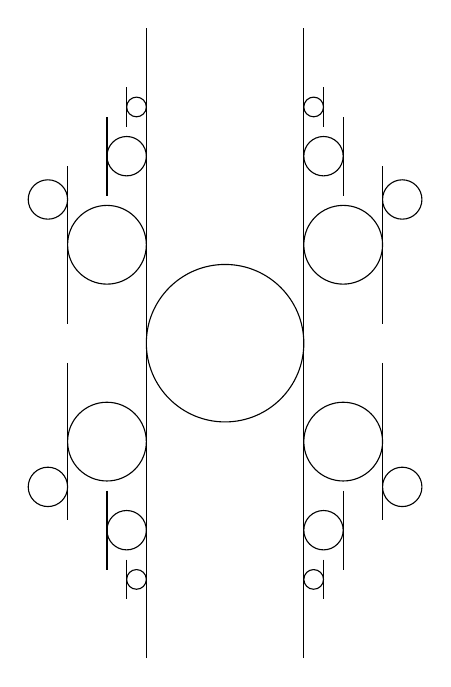
\begin{tikzpicture}
    % FIRST LEVEL
    \draw (-1,-4) -- (-1,4);
    \draw (1,-4) -- (1,4);
    \draw (0,0) circle (1cm);
    % SECOND LEVEL
    % additional circles
    \draw (-1.5,1.25) circle (.5cm);
    \draw (1.5,1.25) circle (.5cm);
    \draw (-1.5,-1.25) circle (.5cm);
    \draw (1.5,-1.25) circle (.5cm);
    % other lines
    \draw (-2,.25) -- (-2,2.25);
    \draw (-2,-.25) -- (-2,-2.25);
    \draw (2,.25) -- (2,2.25);
    \draw (2,-.25) -- (2,-2.25);
    % additional circles
    \draw (-1.25,2.375) circle (.25cm);
    \draw (1.25,2.375) circle (.25cm);
    \draw (-1.25,-2.375) circle (.25cm);
    \draw (1.25,-2.375) circle (.25cm);
    % other lines
    \draw (-1.5,1.875) -- (-1.5,2.875);
    \draw (-1.5,-1.875) -- (-1.5,-2.875);
    \draw (1.5,1.875) -- (1.5,2.875);
    \draw (1.5,-1.875) -- (1.5,-2.875);
     % additional circles
    \draw (-1.125,3) circle (.125cm);
    \draw (1.125,3) circle (.125cm);
    \draw (-1.125,-3) circle (.125cm);
    \draw (1.125,-3) circle (.125cm);
    % other lines
    \draw (-1.25,2.75) -- (-1.25,3.25);
    \draw (-1.25,-2.75) -- (-1.25,-3.25);
    \draw (1.25,2.75) -- (1.25,3.25);
    \draw (1.25,-2.75) -- (1.25,-3.25);
    % THIRD LEVEL
    \draw (-2.25,1.825) circle (.25cm);
    \draw (2.25,1.825) circle (.25cm);
    \draw (-2.25,-1.825) circle (.25cm);
    \draw (2.25,-1.825) circle (.25cm);
    % other lines
    \draw (-1.5,1.875) -- (-1.5,2.875);
    \draw (-1.5,-1.875) -- (-1.5,-2.875);
    \draw (1.5,1.875) -- (1.5,2.875);
    \draw (1.5,-1.875) -- (1.5,-2.875);
  \end{tikzpicture}
  \caption{The Cayley graph of $\Z \ast \Z/2$.}
\end{figure}

\exercise{1.3.31}

The forward direction is clear from the definition: Given a
presentation for a group $G$ with two generators we construct the
space $X_G$ as the wedge of 2 circles as well as 2-cells attached
along the relations in the presentation of $G$. This space has $S^1
\vee S^1$ as a deformation retract. If we let $\tilde{X}_G$ be the
Cayley graph of $G$ then $\tilde{X}/G = X_G$ and when we compose the
covering map with the retraction, we retain the covering map, so
$\tilde{X}$ is a covering space of $S^1\vee S^1$. Moreover,
proposition 1.26 guarantees that the covering space is normal.

In the other direction we are given a normal covering space of
$S^1\vee S^1$ and must show that this is a Cayley graph of some group
on two generators. If $\tilde{X}$ is the normal covering space then we
know by Proposition 1.39 that the group of deck transformations $G(X)
\cong \pi_1(S^1 \vee S^1)/p_*(\pi_1(\tilde{X}))$. We then construct
the Cayley graph of $p_*(\pi_1(\tilde{X}))$ and note that the
construction (c.f. discussion at the top of pg 77) guarantees that the
graph $X_G$ satisfies
\[
X_G \cong \pi_1(S^1 \vee S^1)/p_*(\pi_1(\tilde{X})) \cong G(X)
\]
as desired. The proof of the general case is exactly the same.

\exercise{A1}

If $X$ is Hausdorff and has a compact covering space $p: \tilde{X} \to
X$. Construct an open neighborhood $U_x$ about each $x \in X$. If we
lift each of these into $\tilde{X}$ we get an open cover for
$\tilde{X}$. Because $p^{-1}(U_x)$ is the disjoint union of copies of
$U_x$ we can cover $\tilde{X}$ by a collection of copies of $U_x, x
\in X$. By compactness we can extract a finite subcover,
$\{U_{x_i,k}\}$ and we can take each of these sets to be disjoint
because $X$ is Hausdorff. Because the fibers above each point have the
discrete topology, the finite disjoint cover implies that the fiber
above each point must also be finite. Then because a loop in
$\pi_1(X,x_0)$ lifts to a unique path in $\tilde{X}$ rooted at some
point in $p^{-1}(x_0)$ and the number of such paths is finite we see
that $\pi_1(X,x_0)$ must be finite as well. Because $X$ is path
connected, this does not depend on the choice of $x_0$ and we are
done.

\exercise{A2}

For the first part, consider the binary expansion of each real
number. We construct a family of group presentations as follows:
\begin{enumerate}
\item To each real $r = d_0d_1\ldots$ assign the sequence of groups
  \begin{align*}
    \lbrace a,b &\mid a^{d_0}\rbrace \\
    \lbrace a,b &\mid a^{d_0}b^{d_1}\rbrace \\
    \lbrace a,b &\mid a^{d_0}b^{d_1}a^{d_2}\rbrace \\
    &\vdots
  \end{align*}
\item To construct a bijection from the reals to groups on two
  generators, let $G_r$ be the first group in the sequence for $r$
  that is not isomorphic to $G_\ell$ for any $\ell < r$. We know this
  is possible because the decimal expansion of each distinct reals is
  distinct.
\item Let $\tilde{X}_{G_r}$ be the Cayley graph of $G_r$. We showed in
  a previous problem that each of the $X_{G_r}$ are normal covering
  spaces for $S^1 \vee S^1$.
\end{enumerate}
So we have an injection from $\R$ into the covering spaces of $S^1
\vee S^1$. Because each of these Cayley graphs corresponds to a normal
subgroup of $\pi_1(S^1 \vee S^1) \cong \Z \ast \Z$ we see that the
free group on two generators has uncountabley many subgroups. This is
not true for the free abelian group on two generators. This is an
immediate consequence of the structure theorem for finitely generated
abelian groups (there are only countably many subgroups of $\Z$ and
taking products doesn't increase cardinality for infinite sets).

\exercise{A3}

Given a finitely generated group $G$ and a subgroup $H \leq G$ of
finite index we consider the space $X_G$ which is the two dimensional
cell complex corresponding to $G$ such that $\pi_1(X_G) \cong
G$. Because $G$ is finitely generated, it's 1-skeleton must be
finite. Moreover, because $H$ has finite index in $G$ we apply
Proposition 1.36 to get a covering space $\tilde{X}_G$ of $X_G$ with a
finite 1-skeleton. Moreover, the proposition says $pi_1(\tilde{X}_G)
\cong H$. Because $X_G$ has a finite one skeleton and the orbit space
of $H$ is finite $H$ must also have a fninite 1-skeleton which means
it too is finitely generated.

In the case that $G$ is a finitely presented group and $H \leq G$ has
finite index we follow a similar construction. This time we construct
$X_G$ by attaching a 2-cell along each relation in the presentation
for $G$ and note that if the number of relations is finite, then $G$
has both a finite 1-skeleton and 2-skeleton. Then the construction
above translatees exactly: $H$ induces a covering space that must have
a finite 1 and 2 skeleton and therefore is finitely presented.

For the last part, suppose that $G$ is a finitely generated group with
$n$ generators. In our initial construction of the space $X_G$ we
begin with attaching 1-cells to make loops for each relation and
wedging the loops together. Then the Cayley subgraph of the group $H$
in $X_G$ has $x$ vertices and $nx$ edges if $[H : G] = x$. But then we
can construct a spanning tree of theis graph with $m-1$ edges and so
by Proposition 1A.2 $H$ can have at most $nm - (m-1)$ generators. This
gives that the number or generators for $H$ is at most $m(n-1) + 1$.

\exercise{A4}
\begin{enumerate}
\item[\textbf{(a)}] We know that $\pi_1(\R P^2) \cong \Z/2$, which has
  two subgroups, and so there are two connected covering spaces of $\R
  P^2$. We know that $\R P^2$ itself is a covering space with the
  identity map as the cover, and so the other space must be the two
  sheeted cover $S^2 \to \R P^2$. Consequently, any covering space of
  $\R P^2$ is a disjoint union of some number these spaces.

  Now if we look at the covering spaces of $\R P^2 \vee \R P^2$ we see
  that they must contain copies of covering spaces of $\R P^2$ and
  furthermore, must be they union of covering spaces because if we
  project onto the first coordinate, we are left with a covering space
  of $\R P^2$.

  Let $v$ be the basepoint in $\R P^2 \vee \R P^2$ and now consider a
  neighborhood of $v$. Because this neighborhood must lift to a
  disjoint union of neighborhoods, each homeomorphic to the original,
  we can brute-force the ways that $\R P^2$ and $S^2$ can intersect
  and satisfy this property:
  \begin{enumerate}
  \item We can intersect the poles of the two spheres.
  \item We can intersect to $\R P^2$'s at their basepoints.
  \item We can intersect an $S^2$ and an $\R P^2$ at the pole of the
    former and the basepoint of the latter.
  \end{enumerate}
  Because of the fact that the two spaces correspond to different
  summands in the base space, we can see that they must correspond to
  different edges in the covering space. So this means that we can
  construct a covering space as a wedge of spheres, possibly
  terminated by an $\R P^2$ at the end of any chain. These are all of
  the possibilities.
\item[\textbf{(b)}] We apply the previous part and van Kampen's theorem
  as follows: because $\pi_1(\R P^2) \cong \Z/2$ we see that
  \[
  \pi_1(\R P^2 \vee \R P^2) \cong \pi_1(\R P^2) \ast \pi_1(\R P^2)
  \cong \Z/2 \ast \Z/2
  \]
  We know that each subgroup corresponds to a connected covering space
  of $\Z/2 \ast \Z/2$ and so each of the covering spaces corresponds
  to the following:
  \begin{align*}
  \{1\} &\mapsto \text{ the universal cover} \\
  \lbrace a,b \mid a\rbrace &\mapsto \R P^2 \\
  \lbrace a,b \mid (ab)^n\rbrace &\mapsto \text{ the wedge of spheres} \\
  \lbrace a,b \mid a,(ab)^n\rbrace &\mapsto \text{ the wedge of
    spheres with }\R P^2 \text{ attached}
  \end{align*}
  The other constructions are very similar. We can take the space
  $X_3$ to be a circle corresponding to the generator of $\Z/3$ with a
  2-cell attached along the relation $x^3$ so that $\pi_1(X_3) \cong
  \Z/3$. By the van Kampen, we see that
  \begin{align*}
    \pi_1(\R P^2 \vee X_3) &\cong \Z/2 \ast \Z/3 \\
    \pi_1(X_3 \vee X_3) &\cong \Z/3 \ast \Z/3
  \end{align*}
  By the same reasoning as the case of $\Z/2 \ast \Z/2$ we see that
  there are 6 isomorphism classes of $\Z/2 \ast \Z/3$ and 9 of $\Z/3
  \ast \Z/3$.
\end{enumerate}
\end{document}
